\chapter{Experimental results}\label{ch:basic}

Now that the model has been described, it is time to present
experimental results. The results will be presented in three
forthcoming chapters including this one. The current chapter presents the complete outline of one experiment that will form the basis with which
the results of most other experiments will be compared. This experiment will be called the basic experiment and implements the guessing game.

\chapref{ch:par} will show how some parameters and methods
influence the language game. Some experiments will be discussed
in which the quality of the communication completely breaks
down, but most experiments will show which parameter settings
and methods improve the language game.

Before the experiments are discussed some methodology and measures have
to be defined. This is done in the next section. The physical
recording of the sensory data is discussed in \sectref{s:st:data}. \sectref{s:st:experiment} presents the
basic experiment. Both the effectiveness and evolution will be
discussed. A summary is given in \sectref{basic:summary}.

\section{Measures and methodology}\label{s:st:measures}
\subsection{Measures}

As in any empirical investigation, measures are needed to
monitor the effectiveness of the system. For the experiments
presented here seven measures have been proposed, each measuring
a certain aspect of the system. Three measures monitor the categorisation: {\sc discriminative success}, {\sc
distinctiveness} and {\sc parsimony}. The other four measures
are involved with the quality of the communication system: {\sc
communication success}, {\sc actual success}, {\sc
specificity} and {\sc consistency}. All measures are values between 0 and 1; 0 means complete failure and 1 complete success.

The measures distinctiveness, parsimony, specificity and consistency were introduced by Edwin \citet{dejong:2000}. These measures are based on the entropy measure taken from information theory \citep{shannon:1948}. Entropy measures the uncertainty about a set of elements. The higher the entropy, the higher the uncertainty introducing chaos. Low entropy means order and less uncertainty. Information theory defines entropy as follows:\is{entropy}%\ia{de Jong, Edwin D.}

\begin{quote}
Let $X$ be a random variable with a set of possible outcomes $A_X=\{a_1,\ldots,a_n\}$, having probabilities $P_X=\{p_1,\ldots,p_n\}$ with $P(x=a_i)=p_i$, $0 \leq p_i \leq 1$ and $\sum_{i=1}^n P_i = 1$. Then according to \citet{shannon:1948}, the entropy $H$ of $X$ is defined by:
\begin{eqnarray}
H \equiv -\sum_{i=1}^n P_i \cdot \log P_i
\end{eqnarray}
with the convention for $P_i=0$ that $-0 \cdot \log 0 = 0$. The information theoretic entropy used here should not be confused with entropy in physical systems, as in the second law of thermodynamics, although there is a relation in that both forms of entropy measure disorder \citep[76]{dejong:2000}.
\end{quote}


\noindent All measures that are used can now be described as follows:

\begin{description}
\item[Discriminative success]\is{discriminative success} To monitor the ability of
the robots to discriminate a segment from other segments in the
context, discriminative success {\scshape (ds)} has been introduced \citep{steels:1996b}. At each instance, the discriminative success measures the average
success of an agent to discriminate over the past 100 language
games. Although a robot may play more discrimination games than
language games, it is opted to measure the success over 100
language games for simplicity. So, if during 100 language games
a robot played 120 discrimination games, the discriminative success measures the average
success of those 120 discrimination games. On the other hand, if there are only 80 discrimination games played, the discriminative success monitors the success of these 80 games as a function of the 100 language games. So, the discriminative success
monitors the evolution of categorisation, although its information is not always equally reliable. Note that the discriminative success is calculated for each individual robot.
\item[Distinctiveness]\is{distinctiveness} ``Intuitively, distinctiveness expresses to what degree a meaning identifies the referent.'' \citep{dejong:2000} For this we can measure how the entropy of a meaning in relation to a certain referent $H(\rho|\mu_i)$ decreases the uncertainty about the referent $H(\rho)$. For this we can calculate the difference between $H(\rho)$ and $H(\rho|\mu_i)$. Here $\rho$ are the referents $\rho_1,\ldots,\rho_n$ and $\mu_i$ relates to one of the meanings $\mu_1,\ldots,\mu_m$ for robot $R$. The distinctiveness $D_R$ can now be defined as follows:
\begin{eqnarray}
H(\rho|\mu_i)=\sum_{j=1}^n -P(\rho_j|\mu_i) \cdot \log P(\rho_j|\mu_i)
\end{eqnarray}
\begin{eqnarray}
\mbox{dist}(\mu_i)=\frac{H(\rho)-H(r|\mu_i)}{H(\rho)}=1-\frac{H(\rho|\mu_i)}{H(\rho)}
\end{eqnarray}
\begin{eqnarray}
D_R=\frac{\sum_{i=1}^m P_o(\mu_i) \cdot \mbox{dist}(\mu_i)}{m}
\end{eqnarray}


where $H(\rho)=\log n$ and $P_o(\mu_i)$ is the occurrence probability of meaning $\mu_i$. The use of $P_o(\mu_i)$ as a weighting factor is to scale the importance of such a meaning to its occurrence. In \citet{dejong:2000} this has only been done for specificity and consistency, because there the occurrence of meanings and referents was a normal distribution.

\item[Parsimony]\is{parsimony} The parsimony $P_R$ is calculated similar to the distinctiveness:
\begin{eqnarray}
H(\mu|\rho_i)=\sum_{j=1}^m -P(\mu_j|\rho_i) \cdot \log P(\mu_j|\rho_i)
\end{eqnarray}
\begin{eqnarray}
\mbox{pars}(\rho_i)=1-\frac{H(\mu|\rho_i)}{H(\mu)}
\end{eqnarray}
\begin{eqnarray}
P_R=\frac{\sum_{i=1}^n P_o(\rho_i) \cdot \mbox{pars}(\rho_i)}{n}
\end{eqnarray}


with  $H(\mu)= \log m$. Parsimony thus calculates to what degree a referent gives rise to a unique meaning.

\item[Communicative Success]\is{communicative success} The communication success
{\scshape (cs)} is calculated similar to the discrimination success. communicative success is the average success in communication
over the past 100 games. It must be noted that when a language
game ends in communicative success, the robots not necessarily
communicated the same topic. The robots considered the language
game successful as a result from the feedback. Since the feedback is not always sound, the communicative success does not always say anything about
the robots ability to communicate about a certain referent.

\item[Actual success]\is{actual success} In order to say more about the
actual success of a language game, when the communicative success is not the ideal measure, the measure actual success {\scshape (as)} has been introduced \citep{vogt:1998b}. The actual success
measures the success of a language game as if it were observed
by an objective observer. The objective observer may regard the language game successful when it is so according to the correspondence criterion, i.e., when the topic of both robots correspond to the same light source. This method is not completely sound, because at larger distances to a light source the correspondence criterion is not sound. But in most cases it suffices. The actual success measures the
average success over the past 100 language games. When feedback is provided by the correspondence criterion, the actual success is the same as the communicative success.

\item[Specificity]\is{specificity} ``The specificity of a word[-form] is [...] defined as the relative decrease of uncertainty in determining the referent given a word that was received.'' \citep{dejong:2000} It thus is a measure to indicate how well a word-form can identify a referent. It is calculated analogous to the distinctiveness and parsimony. For a set of word-forms $\sigma_1,\ldots,\sigma_q$, the specificity is defined as follows:
\begin{eqnarray}
H(\rho|\sigma_i)=\sum_{j=1}^n -P(\rho_j|\sigma_i) \cdot \log P(\rho_j|\sigma_i)
\end{eqnarray}
\begin{eqnarray}
\mbox{spec}(\sigma_i)=1-\frac{H(\rho|\sigma_i)}{H(\rho)}
\end{eqnarray}
\begin{eqnarray}
S_R=\frac{\sum_{i=1}^q P_o(\sigma_i) \cdot \mbox{spec}(\sigma_i)}{q}
\end{eqnarray}


where $H(\rho)=\log n$ is defined as before and $P_o$ is the occurrence probability of encountering word-form $\sigma_i$.

\item[Consistency]\is{consistency} Consistency measures how consistent a referent is named by a certain word-form. It is calculated as follows:
\begin{eqnarray}
H(\sigma|\rho_i)=\sum_{j=1}^q -P(\sigma_j|\rho_i) \cdot \log P(\sigma_j|\rho_i)
\end{eqnarray}
\begin{eqnarray}
\mbox{cons}(\rho_i)=1-\frac{H(\sigma|\rho_i)}{H(\sigma)}
\end{eqnarray}
\begin{eqnarray}
C_R=\frac{\sum_{i=1}^n P_o(\rho_i) \cdot \mbox{cons}(\rho_i)}{n}
\end{eqnarray}
where $H(\sigma)=\log q$ and $P_o(\rho_i)$ is defined as before.
\end{description}

Distinctiveness, parsimony, specificity and consistency are all calculated every 200 language games. Obviously calculations can only take place when the pairs referent -- meaning or referent -- word-form are used. This happens either when the discrimination game is successful (influencing distinctiveness and parsimony) or when a robot produced or understood a communication act (influencing specificity and consistency).\footnote{Note that this does not necessarily mean that the language game was successful.}

\subsection{Statistical testing}

Every experiment (unless otherwise mentioned) consists of 10 runs in which either 5,000 or 10,000 language games are played. When appropriate, the results are presented in a plot that displays the average evolution of the experiment. However, to save space, most results are presented in a table where the global averages of an experiment are given. Using global averages means that the average measure of each complete run (5,000 or 10,000 games) is averaged over 10 runs. This average is given with its standard deviation of the population. When comparing to other experiments, the results are usually displayed in a bar chart. In addition, statistical significance testing is done by these comparisons.
	
\is{Mann-Whitney U test}\is{Wilcoxon rank sum test|see{Mann-Whitney U test}} All statistical significance testing is done using the two-tailed Mann--Whitney $U$ test, also known as the Wilcoxon rank-sum test. Applying the Mann--Whitney $U$ test requires that the population does not show a normal distribution. Investigations of the distributions revealed that the populations were not normally distributed. 

The null-hypothesis of the test may be rejected when $p<\alpha$ for some low $\alpha$. In all testing, the null-hypothesis states that two populations of measurements are the same, with the alternative hypothesis that they are not the same. For stating that one result is significantly better than another, the distributions of the two populations of measurements need to be similar. This has not been observed, so the only inference one can make of a low $p$-value is that the two populations are not the same. However, if one measurement is higher than another, the assumption will be made that this is the case if a $p$-value is low. The value $\alpha$ will not be filled in as the reader may decide whether or not the difference is significant. For readers unfamiliar with statistical testing, the literature usually takes $\alpha=0.05$, which becomes $\alpha=0.025$ for a two-tailed test. The used method and tables are taken from \citet{aczel:1989}.

Other methods will be used to evaluate an experiment's success.
These methods include semiotic landscapes, competition diagrams and others, and
will be introduced with their initial appearance.

\subsection{On-board versus off-board}\label{s:lg:offboard}

In the original experiments all the processing, including the meaning and language formation, was done on-board the robots \citep{steelsvogt:1997}. But, since the robots failed to enhance the lexicon due to the lack of on-board memory and because the robots' batteries only work for one hour while the experiments take much more time, a large part of the processing is done off-board on a personal computer. The sensory information that the robots detect during sensing is sent to the {\scshape pc} by the radio link. After the robots recorded the sensory information of a language game, segmentation, categorisation and naming are further processes on the {\scshape pc}. There are many advantages for off-board processing:

\begin{enumerate}
\item Larger internal memory
\item No loss of data during change of batteries
\item Faster processing
\item Repeatable experiments to compare parameter settings and methods more reliably
\item Debugging
\end{enumerate}


After approximately one hour of experimenting, the robot's batteries die. The robots have no persistent data storage on-board. So, when the batteries are empty and the robot shuts down, the memory built up disappears unless it is saved off-board first. Of course, the robots may be powered by a cable, but in practice this proves to be rather cumbersome. The advantage would be that a serial cable can be attached to monitor the internal dynamics of the robots during a game, but this could also be done using radio communication.

The recording of one language game when the robots need to look for each other takes approximately 1.5 min. Recording a minimum of 5,000 language games takes therefore 125 hours, which takes 25 days or 5 weeks assuming that there are 5 effective experimental hours a day.\footnote{Perhaps some robotics researchers laugh at this positive estimation, but in good days this is manageable.} {\em If nothing goes wrong, naturally!} This period can be reduced to 5 days if the researcher manually brings the robots together after which the robots play a series of, say, 10 games in a row. 

Now suppose that one wants to tune a parameter by varying this parameter 5 or 10 times. Or that one wants to change a method, or what if the researcher finds a bug in its program. For all these reasons off-board processing is the outcome. Another important advantage is that one can use the same recordings over and over again across different experiments, so comparing different experiments is more reliable.

Debugging is a good reason to process data as much as possible off-board as well, it saves huge amounts of time. Many more advantages can be found, but the biggest have been stated. However, if one divides a system in on-board vs. off-board processing, then one should be careful to define the division line. The experiment should not loose its embodied and situated character, otherwise one is better off using simulations.

\section{Sensory data}\label{s:st:data}\is{situation}

As mentioned in \chapref{ch:lg} the sensory data of the
sensing during a language game is recorded to further
process the game off-board. For convenience the sensing is segmented in advance, using the method
described in \chapref{ch:lg}. The same is done for the feature extraction. The data set thus consists of
the contexts described by the feature vectors of the two robots participating in the experiment. The two contexts that relate to one language game will be called a {\sc situation}.

For obvious reasons of time, a few data sets of only 1,000
situations have been recorded. One of these sets is used for the experiments of this chapter, the others will be presented in \chapref{ch:par}. As will become clear soon,
an experiment requires approximately 3,000 language
games before the communication system becomes more or less stable. In most experiments 5,000 games are played. In these experiments the
1,000 recorded situations will be used over and over again. Some people may ask if the reuse of situations will bias the system. But it is unlikely that two language games in the experiment are the same.
Every language game one situation is selected. One of the
robots is then randomly assigned to play the role of the
speaker. The speaker then randomly selects one of the segments
to be the topic. Since, on average, each context consists
of approximately 3--4 segments (1017 in the first data set to be
precise), a situation can be used in, say, 7 different ways. Assuming
perfect randomness of the system, each possible setting
(situation, role assignment and topic choice) has been explored only once
after approximately 7,000 games, which justifies this method. 

The data set is first run through linearly, i.e. the system that runs
the experiment reads the data set in recording sequence. 
The situations are stored in a list and each situation is then selected in
random order.

The 1,000 situations have been recorded as described in \chapref{ch:lg}. The recording of each data set took approximately 8 hours of work, spread over two days.

Before the results of the cognitive processing is presented, it is useful to look at some statistics of the basic data set.\is{data set!basic} Some additional statistics of the basic data set are presented in Appendix \ref{a:dataset}. This appendix shows the distribution of the feature values measured by the robots. This distribution shows one reason why it seems impossible that a real-world environment can be simulated.

\tabref{t:st:data} shows the average context size $\langle |Cxt| \rangle$ of each robot together with its standard deviation. In addition, this table shows the {\scshape potential understandability} $U_r$ of each robot.\is{understandability!potential|see{understandability}}\is{understandability|(} The potential understandability of a robot is a measure that indicates how well a robot can be understood by another robot according to their context sharing. Suppose that robot $r$ has segmented context $Cxt_{r,l}=\{S_{1,r,l},\ldots,S_{n,r,l}\}$ for situation $l$, then the understandability $U_r$ for $n$ situations is calculated as follows:
\begin{eqnarray}
U_{r,l}=\frac{\sum_{i=1}^n u_{i,l}}{n}
\end{eqnarray}
where
\begin{eqnarray}
u_{i,l} = \left \{ \begin{array}{rl}
1 & \mbox{if} S_{i,r,l} \sqsubseteq Cxt_{r',l} \; (r \neq r')\\
0 & \mbox{otherwise}
\end{array} \right.
\end{eqnarray}
\begin{eqnarray}
U_r = \frac{\sum_{l=1}^L U_{r,l}}{L}
\end{eqnarray}
\noindent where the symbol $\sqsubseteq$ is used to denote the relation whether the segment on the left hand side of $\sqsubseteq$ corresponds to one of the segments in the context of the other robot. $L$ is the total number of situations recorded. So, the global potential understandability $U_r$ is the average of the average potential understandability per situation. In \tabref{t:st:data} this average is given with its standard deviation.

The potential understandability is lower than 1, because the two robots do not always share a similar context. That this happens has already been discussed in the preceding \chapref{ch:lg}.

\begin{table}[t]
\centering
\begin{tabular}{rd{3}@{~}c@{~}d{3}c@{~}d{3}@{~}c@{~}d{3}}
\lsptoprule
 & \multicolumn{3}{c}{$r0$} & & \multicolumn{3}{c}{$r1$}\\\midrule
$\langle|Cxt|\rangle$ & 3.33 & $\pm$ & 1.07 & & 3.54 & $\pm$ & 1.21\\
$U_r$ & 0.81 & $\pm$ & 0.27 & & 0.78 & $\pm$ & 0.27\\
\lspbottomrule
\end{tabular}
\caption{The average context size $\langle|Cxt|\rangle$ and average potential understandability $U_r$ of the recorded data set.}
\label{t:st:data}
\end{table}
\is{understandability|)}


What can be expected in the experiments when observing the statistics of this data set? The first thing that can be said is that the a priori probabilities that both robots select the same topic based on the average context size is:\is{a priori success}

\begin{eqnarray*}
P=\frac{\langle|Cxt_{r0}|\rangle+\langle|Cxt_{r1}|\rangle}{2}\cdot \frac{1}{\langle|Cxt_{r0}|\rangle} \cdot \frac{1}{\langle|Cxt_{r1}|\rangle}=0.29
\end{eqnarray*}


So, if the robots perform better than 30 \% in their communicative success, they are actually learning a meaningful language. The second observation that can be made is that it is impossible to reach a communicative success of 100 \% since the robots are in principle not capable of understanding each utterance given the current context setting. They are not likely to perform better than approximately 80 \%, as has been calculated from the potential understandability.\is{understandability} Third, it is likely that the robots will learn to name L0 better than others, since this light source is detected most often. Given these expectations and conclusions it is time to see how the robots do in the language formation.


\section{The basic experiment}\label{s:st:experiment}
\is{basic experiment}

This first experiment will be referred to as the basic experiment. It is called so because this experiment will serve as the basic experiment from which parameters and methods are changed to investigate their influence. That it is not the best experiment will be shown in subsequent chapters.

The experiment is a guessing game with feedback obtained by means of {\scshape correspondence} (see \sectref{s:cm:feedback}).\is{correspondence}

\tabref{t:st:param} shows the parameter settings of the most important variables that have been introduced in \chapref{ch:lg}. Unless otherwise mentioned, the parameters are not changed in the different experiments.

\begin{table}[t]
\centering
\begin{tabular}{ld{-1}}
\lsptoprule
Par & \multicolumn{1}{c}{Value}\\\midrule
$\delta$ & 0.10\\%\hline
$\eta$ & 0.99\\%\hline
$P_s$ & 0.02\\%\hline
$P_h$ & 1.00\\%\hline
\lspbottomrule
\end{tabular}
\caption{Parameters of the system. The parameters include the step-size $\delta$ by which the categories shift towards an observation, the learning rate $\eta$ controlling the adaptation of scores, the creation probability $P_s$ by which the speaker may invent new word-forms, the adoption probability $P_h$ by which the hearer may adopt a new word-form when it does not find a matching word-form with an associated meaning it also categorised, and the success threshold $\Theta_F$ by which the success of a language game may be accepted.\is{form!creation probability}\is{learning rate}}
\label{t:st:param}
\end{table}

\subsection{The global evolution}

\begin{figure}
\centering
\subfigure[CS]{\includegraphics[width=.45\textwidth]{basic/cs.eps}}
\subfigure[DS]{\includegraphics[width=.45\textwidth]{basic/ds.eps}}\\
\subfigure[S]{\includegraphics[width=.45\textwidth]{basic/spec.eps}}
\subfigure[D]{\includegraphics[width=.45\textwidth]{basic/dist.eps}}\\
\subfigure[C]{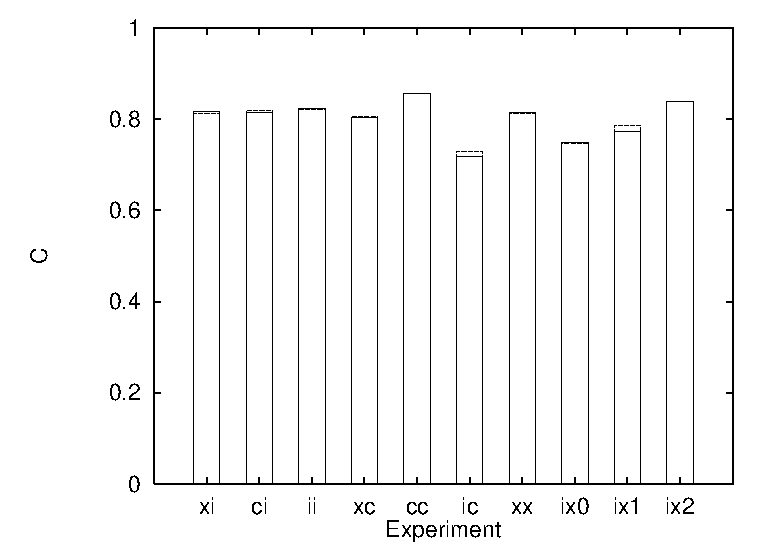
\includegraphics[width=.45\textwidth]{basic/cons.eps}}
\subfigure[P]{\includegraphics[width=.45\textwidth]{basic/pars.eps}}
\caption{The results of the basic experiment showing (a) the communicative success, (b) discriminative success, (c) specificity, (d) distinctiveness, (e) consistency and (f) parsimony. Objective success is not shown, because in this experiment it holds no value (see text).}
\label{f:st:plot}
\end{figure}


The results of the experiment are shown in \figref{f:st:plot}. Note that the actual success is not shown. This is because the actual success is calculated under the same criteria as the feedback of the language games, namely the correspondence criterion. Therefore the actual success is equal to the communicative success. In the experiments where the feedback is provided using the correspondence criterion, the plot of the actual success will not be provided.

In \figref{f:st:plot} (a) the evolution of the communicative success is shown. The communicative success first increases rapidly towards a value of 0.2 after 500 language games, then the communicative success slowly grows to a value of 0.45 after approximately 5,000 language games. The low success is partly due to the relatively poor performance the robots' physical behaviour. This poor behaviour causes the robots to acquire an incoherent context, so a completely successful system cannot emerge. However, the potential understandability predicts a maximum success 80 \%. So this cannot explain why the success stays around 40 \% in the last 3,000 games. Note however that the success is still increasing, but the success stabilises around 55 \% after approximately 8,000 games, as will be shown in \sectref{s:st:10000}. Although the communicative success is low, some important observations can be made when a closer look is taken at the evolution of the communication system. This is done from \sectref{s:basic:comp}.

\is{discrimination game}
\figref{f:st:plot} (b) plots the discriminative success of the two robots $r0$ and $r1$. As can be seen, the discriminative success grows to a value around 95 \%. This success rate is reached quite rapidly. Already after approximately 500 language games a success larger than 90 \% is achieved. That the discriminative success does not converge to 100 \% is due to (1) the hearer does not play a discrimination game in all language games and the discriminative success is a function of the language games, and, (2) a success-rate of 100 \% can never be reached. This latter finding is due to the fact that on the average about 0.5 \% of the segments in one context are the same. 

\figref{f:st:ds} shows the discriminative success of an experiment where all possible configurations are used in the discrimination games. The robots interacted as if they were playing language games, only they did not communicate. The speaker only categorised its selected topic, the hearer categorised all its detected segments. Note that more discrimination games are played than when the robots also communicate, since the hearer only plays a discrimination game when it receives an uttered word-form. Furthermore, since each agent plays a discrimination game every language game, the discriminative success is independent of the language games. The average distinctive success over 10 runs of 5,000 language games is $0.984 \pm 0.001$ for robot $r0$ and $0.987 \pm 0.000$ for $r1$. Due to limitations of the implementation it is difficult to extract all possible configurations, so these experiments are not used for language formation.

Figures \ref{f:st:plot} (c) and (e) show that the specificity and consistency is rather good. When a communication act establishes, whether or not it is successful,\footnote{A communication act is established when the speaker produced an utterance and when the hearer found a matching {\scshape wm} association. This is independent of successful communication.} the robots' utterances specify the referents pretty well and they are also pretty consistent in naming the referent. So, in principle they mastered a good communication system.

The meanings that are used almost uniquely identify a particular referent. This can be seen in \figref{f:st:plot} (d), which shows the distinctiveness of the two robots. When the robots are able to discriminate a segment corresponding to some referent, they do so rather parsimonious (i.e. they tend to use the same meanings), but not very well. The parsimony (\figref{f:st:plot} (f)) is around 0.85. 

So, when the robots are successful in communicating and categorisation, they do so with high accuracy and invariance. \tabref{t:st:averages} shows the average (Avg) scores of the different measures over 10 runs of the complete experiments. All scores given with their standard deviation of the averages over the {\em population} of 10 runs. In forthcoming experiments tables and bar charts with the average scores will be the main comparison source. Plots like in \figref{f:st:plot} will only be used when it is useful to make a certain point.

In \figref{f:st:cs0} the communicative success of one run is shown. It is obvious that this run shows a different evolution than the averaged evolution, as has been shown in \figref{f:st:plot}. The next section will discuss the evolution of the run for which the communicative success has just been shown.

\begin{table}
\centering
\begin{tabular}{ld{4}@{ }c@{ }d{4}} % @{~} adds a forced space between columns.
\lsptoprule
Score & \multicolumn{3}{c}{Avg}\\\midrule
CS & 0.351 & $\pm$ & 0.010\\%\hline
DS0 & 0.916 & $\pm$ & 0.004\\%\hline
DS1 & 0.920 & $\pm$ & 0.004\\%\hline
D0 & 0.956 & $\pm$ & 0.002\\%\hline
D1 & 0.955 & $\pm$ & 0.002\\%\hline
P0 & 0.852 & $\pm$ & 0.004\\%\hline
P1 & 0.851 & $\pm$ & 0.002\\%\hline
S0 & 0.822 & $\pm$ & 0.017\\%\hline
S1 & 0.817 & $\pm$ & 0.011\\%\hline
C0 & 0.816 & $\pm$ & 0.008\\%\hline
C1 & 0.811 & $\pm$ & 0.007\\%\hline
\lspbottomrule
\end{tabular}
\caption{The table listing the average scores for the different measures. The suffix 0 or 1 indicates from which robot the score is ($r0$ or $r1$). The second column gives the global average of the experiment, together  with its standard deviation over the population of 10 runs.}
\label{t:st:averages}
\end{table}

\begin{figure}[p]
\centerline{\includegraphics[width=9cm]{basic/cs0.eps}}
\caption{The communicative success of one run. The evolution shows a fast increase towards 30 \%, after which it slowly grows to 50 \% at the end. The evolution further shows a lot of fluctuations. Apparently the robots learn to communicate with ups and downs. A lot of these fluctuations are caused by polysemy and synonymy in the system as will become clear hereafter.}
\label{f:st:cs0}
\end{figure}
\begin{figure}[p]
	\centerline{\includegraphics[width=9cm]{basic/dsall.eps}}
	\caption{The discriminative success of 10 runs of 5,000 language games in which only discrimination games were played (i.e. without communication). The discrimination games here considered all possible configurations of categories in their contexts.}
	\label{f:st:ds}
\end{figure}

\clearpage
\subsection{The ontological development}\label{s:cat:evol}
\is{prototype!dynamics|(}
\is{prototype|(}
\is{ontology}
It is interesting to see how the ontology of prototypical categories develop and evolve in time.

\begin{figure}
\centering
\subfigure[WL0-1]{\includegraphics[width=.45\textwidth]{categorization/cats0-1.eps}}
\subfigure[WL0-2]{\includegraphics[width=.45\textwidth]{categorization/cats0-2.eps}}\\
\subfigure[WL0-3]{\includegraphics[width=.45\textwidth]{categorization/cats0-3.eps}}
\subfigure[WL0-4]{\includegraphics[width=.45\textwidth]{categorization/cats0-4.eps}}
\caption{The development of prototypes in dimension WL0 of feature spaces ${\mathcal F}_1$ to ${\mathcal F}_4$. Note that the x-axis shows the number of language games and the y-axis shows the value of the prototype in dimension WL0. Similar evolutions are observed in the other dimensions of the feature spaces.}
\label{f:cat:evol1}
\end{figure}

\figref{f:cat:evol1} shows the evolution of prototypes in dimension {\scshape wl\oldstylenums{0}} of feature spaces ${\mathcal F}_1$ to ${\mathcal F}_4$. Similar development is observed for the other dimensions. Recall that each feature space ${\mathcal F}_\lambda$ allows a maximum of $3^\lambda$ exploitations in each dimension. The first exploitations in the different feature spaces are constructed quite rapidly. It is interesting to note that only the prototypes of feature space ${\mathcal F}_1$  are continuously changing (\figref{f:cat:evol1} (a)). This means that they are used successfully to name a segment and shift towards the feature they categorised. The lower and upper exploitations remain close to 0 and 1, respectively, the middle values shift toward values somewhere in the middle between 0 and 1. The categories have the tendency to move towards what could be called the central tendency of the features for which the prototypical categories have been used successfully in the language games. 

At the other feature spaces from \figref{f:cat:evol1}, an increasing amount of prototypes are constructed, but once they are introduced they hardly change. Apparently, these prototypical categories are not often used successfully in the language games. So, the robots appear to be sufficiently effective with the categories constructed in feature space ${\mathcal F}_1$. This does not mean that in a more complex environment, the further refinements would not be effective.

\begin{table}
\centering
\begin{tabular}{rr}
\lsptoprule
M5 & $(0.02, 0.01, 1.00, 0.02)_1$\\%\hline
M6 & $(0.04, 0.00, 0.00, 0.00)_2$\\%\hline
M18 & $(0.56, 0.99, 0.02, 0.02)_1$\\%\hline
M20 & $(0.02, 0.01, 1.00, 0.44)_1$\\%\hline
M27 & $(0.02, 0.31, 1.00, 0.44)_1$\\%\hline
M30 & $(0.02, 0.99, 0.02, 0.02)_1$\\%\hline
M37 & $(0.00, 0.00, 0.00, 0.00)_3$\\%\hline
M53 & $(1.00, 0.01, 0.02, 0.02)_1$\\%\hline
M55 & $(1.00, 0.31, 0.02, 0.02)_1$\\%\hline
M58 & $(0.02, 0.01, 0.30, 0.99)_1$\\%\hline
M61 & $(0.02, 0.01, 0.02, 0.99)_1$\\%\hline
M67 & $(1.00, 0.99, 0.02, 0.02)_1$\\%\hline
M90 & $(0.00, 0.00, 0.01, 0.00)_5$\\%\hline
M393 & $(0.00, 0.00, 0.00, 0.01)_4$\\%\hline
M394 & $(0.00, 0.00, 0.00, 0.01)_5$\\%\hline
\lspbottomrule
\end{tabular}
\caption{The legend of some of the meanings represented by their prototypes. The subscript indicates the feature space ${\mathcal F}_\lambda$ at which the prototypes are stored. The given meanings are taken from the ontology after 5,000 language games.}
\label{t:st:legend}
\end{table}


\tabref{t:st:legend} gives a sample of some meanings that are present in the competition diagrams. An additional legend can be found in Appendix \ref{a:lexicon}. Each meaning is a set of categories of which the values are given in a vector notation. So, the category is a 4 dimensional prototype of the (4 dimensional) segment. The first dimension corresponds with sensory channel {\scshape wl}\oldstylenums{0} (the lowest light sensor), etc. The subscript index indicates feature space at which the categories are stored. Most prototypes have a value of 1 (or 0.99) at the dimension that corresponds to the referent for which they are mostly used. 

There are some exceptions, like for \textsc{m\oldstylenums{6}}, \textsc{m\oldstylenums{37}}, \textsc{m\oldstylenums{90}}, \textsc{m\oldstylenums{393}} and \textsc{m\oldstylenums{394}}, which have all values of (almost) 0. These meanings are used in the beginning of the experiment in which a certain feature space is explored. The relating categories were distinctive, despite the low values in each dimension, because the other segments in the context were categorised with other categories at sensory channels that had higher values in another dimension.

An interesting meaning is {\scshape m}\oldstylenums{67}, which has low distinctiveness. This meaning is used both in relation to light sources \textsc{l}\oldstylenums{0} and \textsc{l}\oldstylenums{1}. \tabref{t:st:legend} explains why. The prototype has high values for both dimension {\scshape wl}\oldstylenums{0} and {\scshape wl}\oldstylenums{1}. If a light source is sensed from a large distance, the sensory channel adjacent to the corresponding sensory channel, both sensory channels may detect intensities close to each other, conform the characteristics shown in \chapref{ch:robots}. After feature extraction, the feature vector has high values in these dimensions. Hence meaning {\scshape m}\oldstylenums{67} might be activated. 

Meanings {\scshape m}\oldstylenums{53}, {\scshape m}\oldstylenums{55} (both \textsc{l}\oldstylenums{0}), {\scshape m}\oldstylenums{18}, {\scshape m}\oldstylenums{30} (\textsc{l}\oldstylenums{1}), {\scshape m}\oldstylenums{5}, {\scshape m}\oldstylenums{20}, {\scshape m}\oldstylenums{27} (\textsc{l}\oldstylenums{2}), {\scshape m}\oldstylenums{58} and {\scshape m}\oldstylenums{61} (\textsc{l}\oldstylenums{3}) all have values of 0.99 or 1.00 in the corresponding dimensions.  So, the discrimination process clearly selects the invariant property of correspondence. The meanings that have values of 0.99 in one dimension of their prototypes are used successfully to categorise a feature vector that has a value lower than 1 in this dimension. In such cases the prototypes evolve to a value lower than 1 since it shifts towards the feature vector. If this prototype would be used only to categorise feature vectors with value 1 in some dimension, this dimension will end up with value of 1.

\is{prototype!dynamics|)}
\is{prototype|)}
\is{ontology|)}

\subsection{Competition diagrams}\label{s:basic:comp}
\is{competition diagram|(}

Up to now only superficial measures have been presented, which already gave useful information on the quality of the emerged communication system. Although the communicative success is low, the system is performing better than chance and a reasonable system seems to have emerged. There is another way of looking at the system that emerged, namely by inspecting so called {\sc competition diagrams}. A competition diagram takes one entity at its basis (e.g. a referent) and shows which elements of another entity (e.g. meanings or word-forms) compete to mean or name this basis.

\figref{f:st:compRC} shows the competition diagram with the referents at the basis and the meanings as the competitors, or in short the referent-meaning {\scshape (rm)} diagram. All plots in this figure show the competition diagrams of robot $r0$ for each referent \textsc{l}\oldstylenums{0}, \textsc{l}\oldstylenums{1}, \textsc{l}\oldstylenums{2} and \textsc{l}\oldstylenums{3}. Each plot shows the relative frequency of the co-occurrence of the meaning with the referent, where the referent is taken as the basis to which the frequencies are compared. These relative frequencies are calculated every 200 language games. A co-occurrence of meanings and referents does not imply they were successfully used. It is obvious that each referent has been categorised by different meanings, although each referent has a clear winning meaning. Hence there is a one-to-many relation between referent and meaning.

\begin{figure}[t]
\centering
\subfigure[L0]{\includegraphics[width=.45\textwidth]{basic/RC0-0.eps}}
\subfigure[L1]{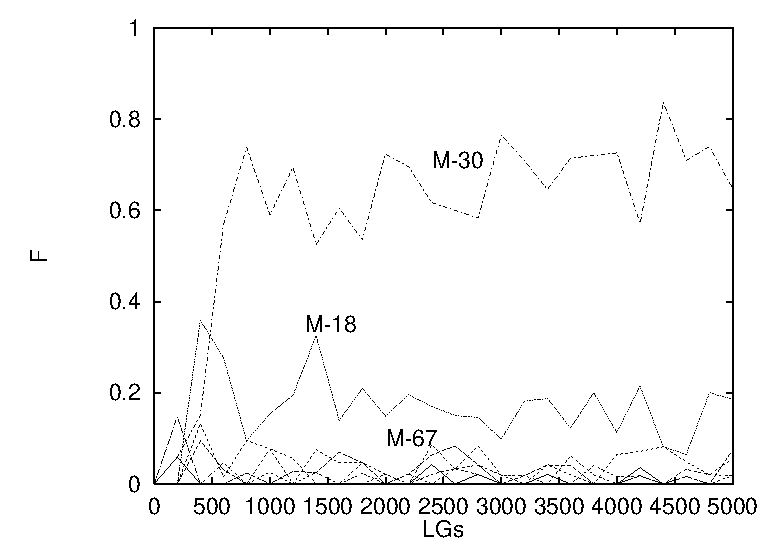
\includegraphics[width=.45\textwidth]{basic/RC0-1.eps}}\\
\subfigure[L2]{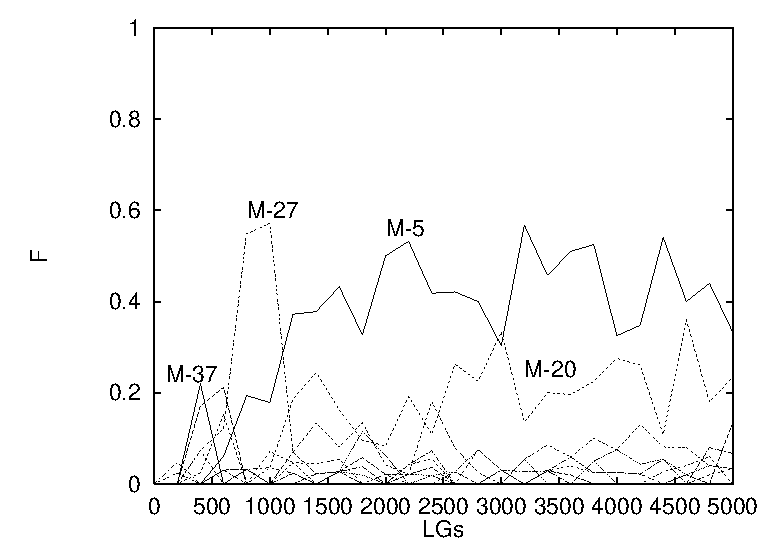
\includegraphics[width=.45\textwidth]{basic/RC0-2.eps}}
\subfigure[L3]{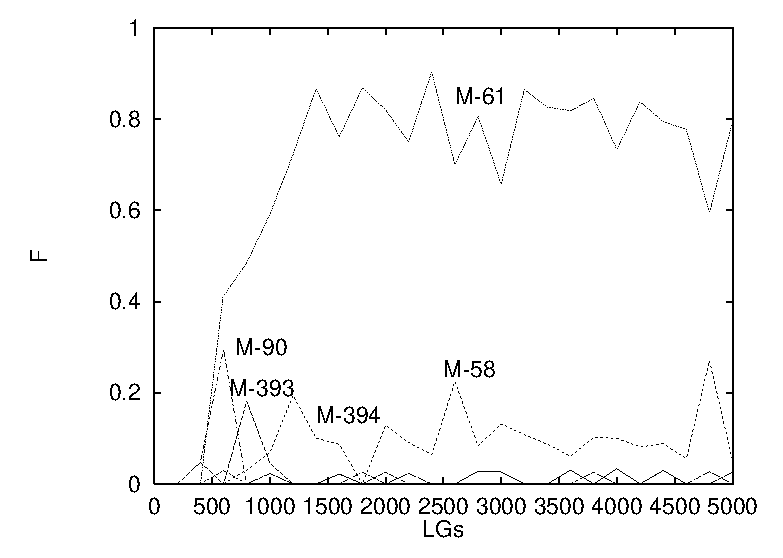
\includegraphics[width=.45\textwidth]{basic/RC0-3.eps}}
\caption{Competition diagrams referent-meaning (or {\scshape rm} diagram).}
\label{f:st:compRC}
\end{figure}


All frequently used meanings are active at feature space ${\mathcal F}_1$ (see also \tabref{t:st:legend}). It appears that, mostly the discrimination is successful using meanings from this feature space.\footnote{Note that categories from feature space ${\mathcal F}_0$ cannot be distinctive unless there is only one segment in the context.} Although this is not shown here, meanings from a feature space with $\lambda>1$ tend not to be used much. Obviously they may just as well be distinctive, but they are not used in the communication, otherwise they would move in the feature space. That this is not the case is observed in \figref{f:cat:evol1}. So, at higher feature spaces, there are more prototypes, but those are selected less frequently. This makes their competition for the referent harder and less successful.

The occurrence frequency of meanings {\scshape m}\oldstylenums{53}, {\scshape m}\oldstylenums{30}, {\scshape m}\oldstylenums{5} and {\scshape m}\oldstylenums{61} constitute the parsimony of the system. It can be inferred that referents \textsc{l}\oldstylenums{0}, \textsc{l}\oldstylenums{1} and \textsc{l}\oldstylenums{3} have a relative high parsimony, whereas \textsc{l}\oldstylenums{2} has relative low parsimony. The higher the parsimony the better a referent is categorised by a single category.

\begin{figure}
\centering
\subfigure[M53]{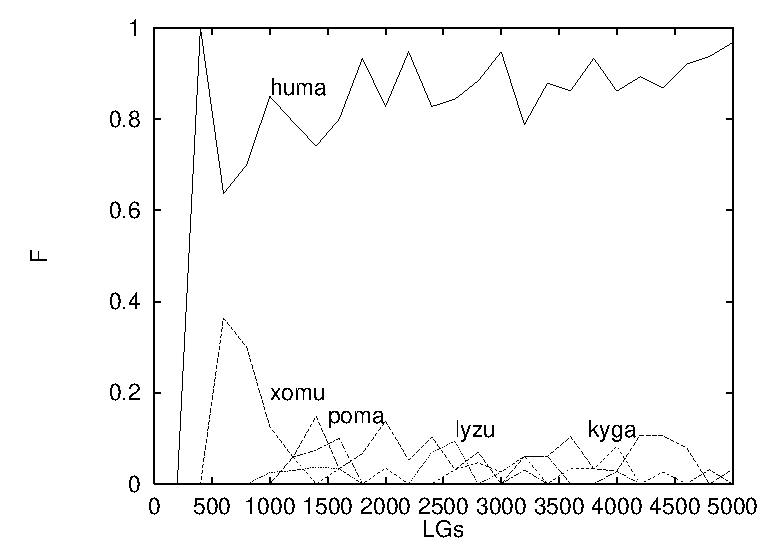
\includegraphics[width=.45\textwidth]{basic/CF0-53.eps}}
\subfigure[M30]{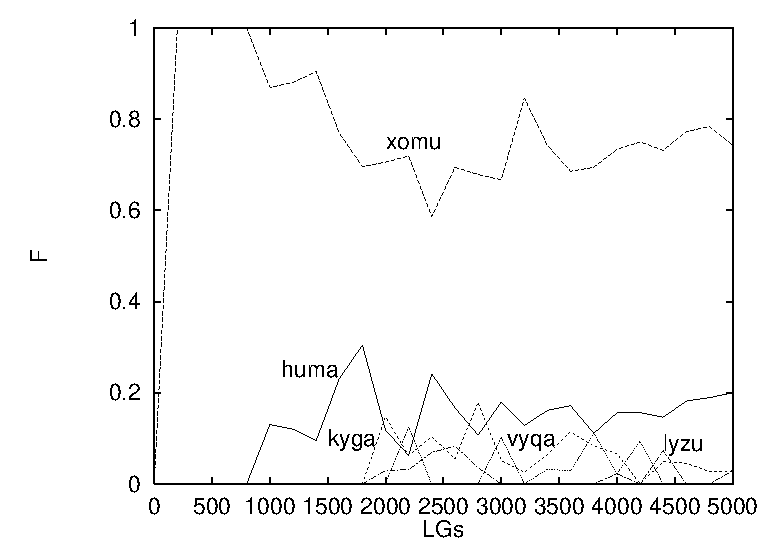
\includegraphics[width=.45\textwidth]{basic/CF0-30.eps}}\\
\subfigure[M5]{\includegraphics[width=.45\textwidth]{basic/CF0-5.eps}}
\subfigure[M61]{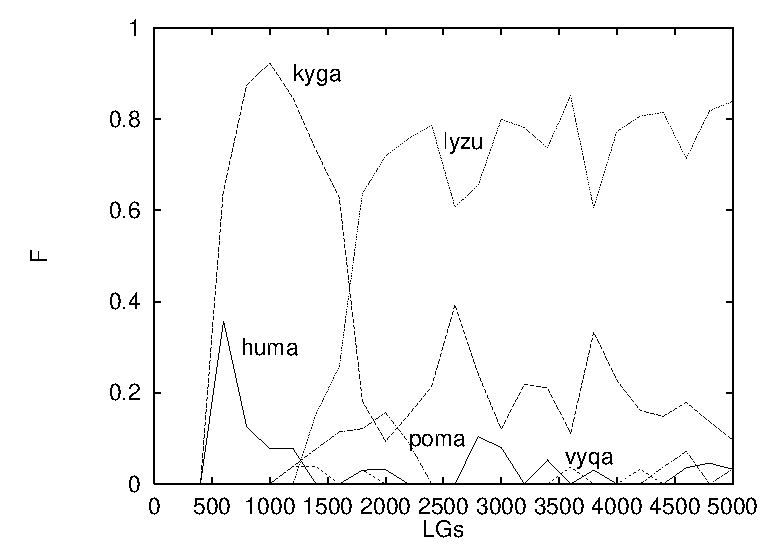
\includegraphics[width=.45\textwidth]{basic/CF0-61.eps}}\\
\subfigure[huma]{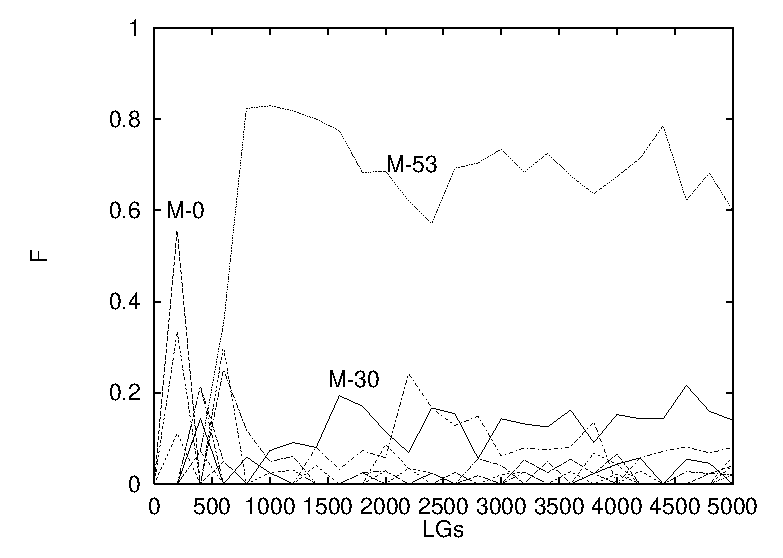
\includegraphics[width=.45\textwidth]{basic/FC0-0.eps}}
\caption{Competition diagrams (a) to (d) meaning-form {\scshape (mf)}, and (e) form-meaning \textsc{(fm)}.}
\label{f:st:compCF}
\end{figure}


Figures \ref{f:st:compCF} (a)--(d) show the meaning-form competition diagrams ({\scshape mf} diagrams) of the winning meanings in the referent-meaning competitions. Figure (a) shows the competition of meaning {\scshape m}\oldstylenums{53}. The word-form {\it huma} clearly wins the competition right from the beginning. Little competition is given by {\it xomu}, {\it poma}, {\it lyzu} and {\it kyga}. Similar competitions can be seen with meanings {\scshape m}\oldstylenums{30} and {\scshape m}\oldstylenums{5} (Figures \ref{f:st:compCF} b and c). So, every meaning shows one-to-many relations between meaning and form. This is highest in for {\scshape m}\oldstylenums{30} and {\scshape m}\oldstylenums{61}. Such one-to-many relations are fed by mismatches that arise in the communication. The mismatches cause word-form adoption, so that a meaning can be associated with several word-forms. The mismatches are mainly due to the rather high level of one-to-many relations between referent and meaning as shown in the referent-meaning diagram. 

The dynamics on the association scores allow the different other lexical elements a chance to compete. Lateral inhibition of competing associations is a main ingredient of the self-organising effect that one element wins the competition. Note again that occurrence in the competition diagram does not equal a language game's success.

Meaning {\scshape m}\oldstylenums{61} (\figref{f:st:compCF} d) shows a different competition than {\scshape m}\oldstylenums{53}, {\scshape m}\oldstylenums{30} and {\scshape m}\oldstylenums{5}. Initially word-form {\it kyga} wins the competition. This word-form is also the winning competitor for {\scshape m}\oldstylenums{5}, so there is representational polysemy in the system. After game 1750 or so, word-form {\it lyzu} starts to win the competition for {\scshape m}\oldstylenums{61} and {\it kyga} is then solely used for {\scshape m}\oldstylenums{5}. Thus the lexicon is somewhat disambiguated. Disambiguation is established by excitation of scores of successful association and the lateral inhibition of competing associations.

\figref{f:st:compCF} (e) shows the opposite competition of form {\it huma} with its associated meanings, i.e., it shows the form-meaning competition for {\it huma}. Again there is a clear winner, namely {\scshape m}\oldstylenums{53} as would be expected. Furthermore some small competition is observed from other meanings. Notably is meaning {\scshape m}\oldstylenums{30}, which is `the best of the rest'. {\scshape m}\oldstylenums{30} is winning competitor referring to {\scshape l}\oldstylenums{1} (see Figures \ref{f:st:compRC} b and \ref{f:st:compCF} b). In \figref{f:st:compCF} (b) {\it huma} also wins the competition of the meanings that are not used for {\scshape l}\oldstylenums{1}, compare \figref{f:st:compRC}.  The form {\it huma} is also used for naming {\scshape m}\oldstylenums{5}, {\scshape m}\oldstylenums{30} and {\scshape m}\oldstylenums{61}, although in a lesser extend. So, there is a one-to-many relation between {\it huma} and some meanings, and there is polysemy is present for {\it huma}. Polysemy means that there are one-to-many relations between the form and referent. Polysemy is one of the causes why the communicative success is lower than the potential communicative success.\is{polysemy}\is{synonymy}

\begin{figure}[t]
\centering
\subfigure[L0]{\includegraphics[width=.45\textwidth]{basic/RF0-0.eps}}
\subfigure[huma]{\includegraphics[width=.45\textwidth]{basic/FR0-0.eps}}\\
\subfigure[M53]{\includegraphics[width=.45\textwidth]{basic/CR0-53.eps}}
\subfigure[M67]{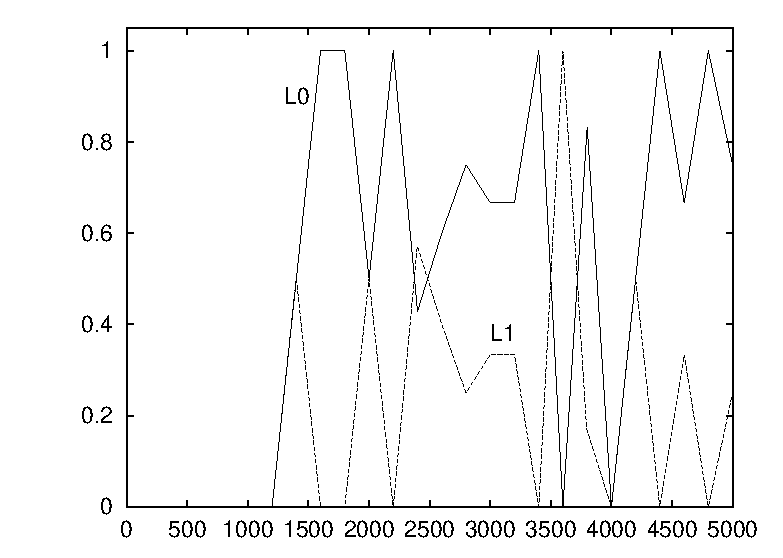
\includegraphics[width=.45\textwidth]{basic/CR0-67.eps}}
\caption{Competition diagrams (a) referent-form, (b) form-referent, (c) and (d) meaning-referent. Meaning {\scshape m}\oldstylenums{53} (c) uniquely refers to referent {\scshape l}\oldstylenums{0}.}
\label{f:st:comp}
\end{figure}

\enlargethispage{1\baselineskip}In \figref{f:st:comp} some different competition diagrams are shown. Figure (a) shows the referent-form competition for {\scshape l}\oldstylenums{0}. The synonymy (one-to-many relation between referent and form) is high, as can be inferred from the low relative frequency of winning word-form {\it huma} and the competing elements at the bottom of the plot. Note that not all competitors are shown in this plot. There are quite some more, but these have lower frequencies than the ones that are shown. The synonymy is a result of the relatively low parsimony (i.e. one-to-many relations between referent and meaning) combined with the one-to-many relations between meaning and form. Naturally, synonymy is an antagonising force against the communicative success.\is{synonymy}

Polysemy of the word-form {\it huma} is also shown in \figref{f:st:comp} (b). At first there is competition between all referents. After 1,000 language games, the tendency to use {\it huma} for naming {\scshape l}\oldstylenums{0} wins the competition. Thus influencing the specificity positively. However, the polysemy antagonises the communicative success. Polysemy is caused by a combination of one-to-many relations between form and meaning and one-to-one relations between meaning and referent, cf. \figref{f:st:comp} (c).

Distinctiveness is high, as can be seen in the meaning-referent diagram for {\scshape m}\oldstylenums{53} (\figref{f:st:comp} c). The relative frequency in using {\scshape m}\oldstylenums{53} for referring to {\scshape l}\oldstylenums{0} goes to 1 where it remains. Some meanings have lower distinctiveness like {\scshape m}\oldstylenums{61} (\figref{f:st:comp} d), which after its introduction around language game 1,200 keeps on competing between {\scshape l}\oldstylenums{0} and {\scshape l}\oldstylenums{1}. That this competition has little influence in the global distinctiveness of robot $r0$ is seen in \figref{f:st:plot} (d). This is so because the occurrence frequency of {\scshape m}\oldstylenums{67} is relatively low.
\is{competition diagram|)}

\subsection{The lexicon}
\is{lexicon|(}

One way of inspecting the resulting lexicon is looking at the competition diagrams. Another way of presenting the lexicon is a table. In such tables word-meaning associations of the two robots are given. Although such tables give good information about an individual's lexicon, it provides difficult to read and incomplete information about its structure in the language using society. Similar tables can display the ontology of the robots in relation to their use for referents. The tables of the lexicon and ontology are given in Appendix \ref{a:lexicon}.

\subsubsection{Semiotic landscape}

\begin{figure}
\centerline{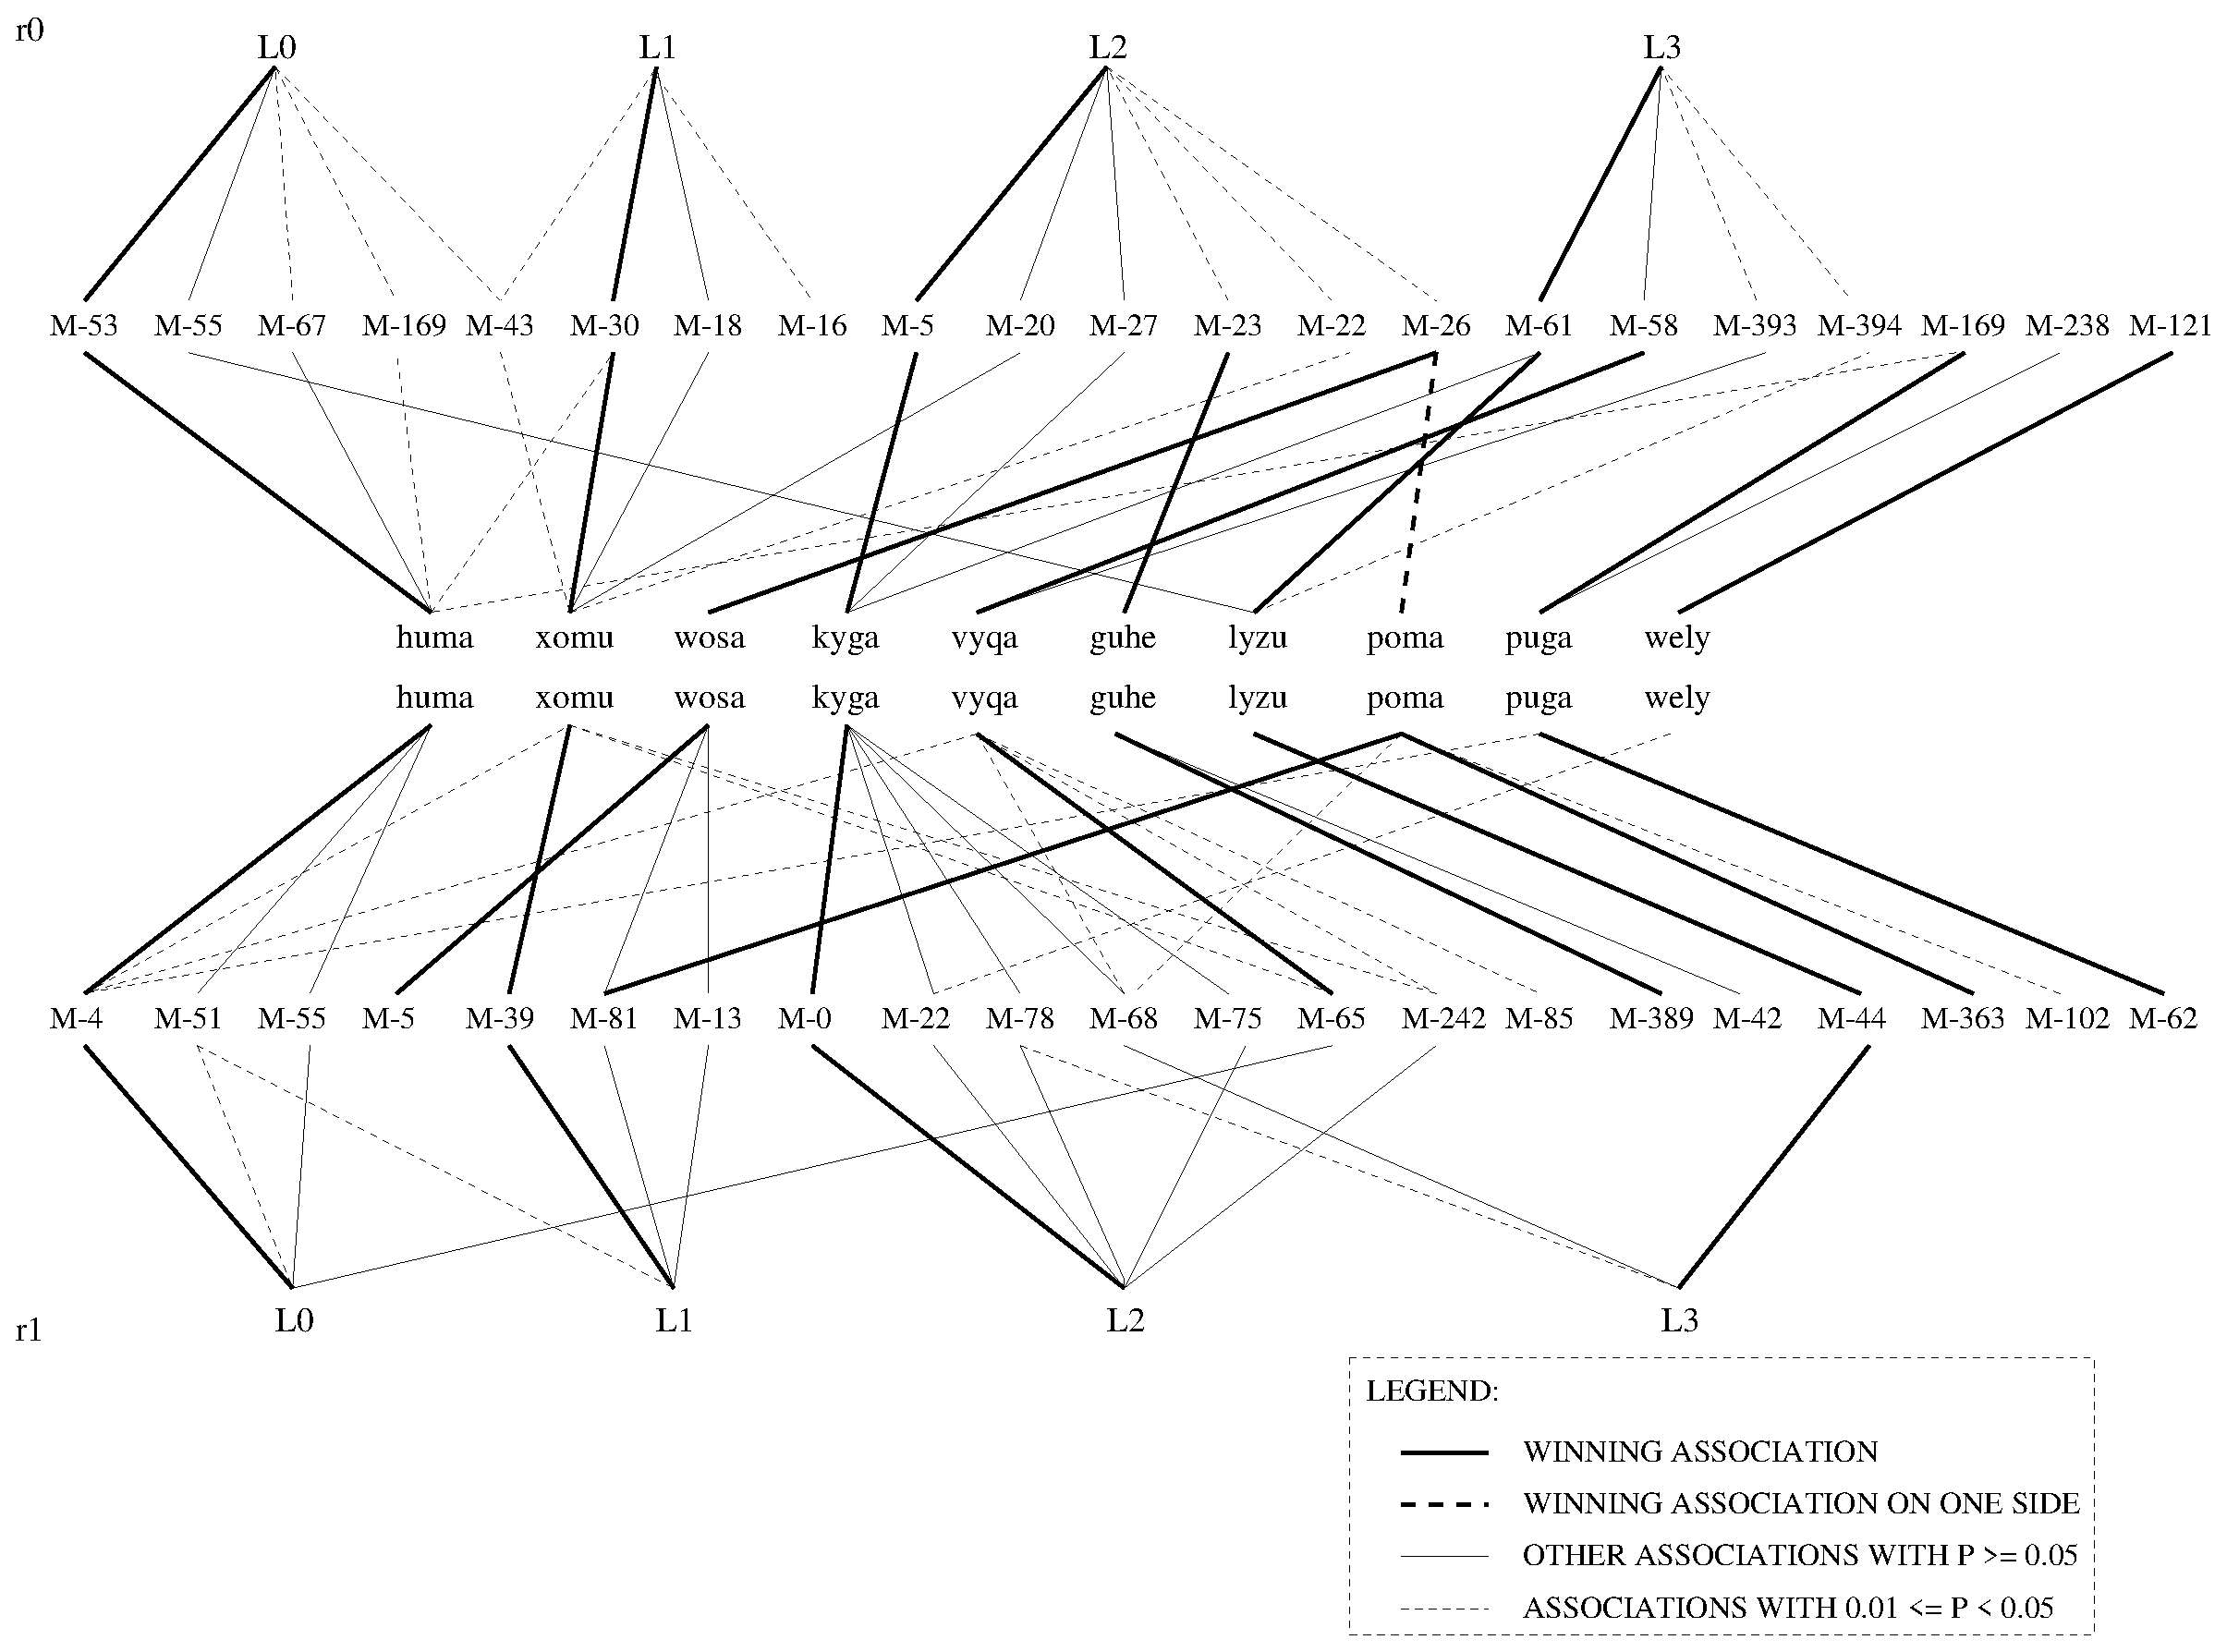
\includegraphics[width=\textwidth]{basic/semiotic.eps}}
\caption{The semiotic landscape of one of the experiments.\is{semiotic landscape}}
\label{f:st:semiotic}
\end{figure}\is{semiotic landscape}

Still another way the lexicon can be presented is by a semiotic landscape as in \figref{f:st:semiotic}. In a semiotic landscape the semiotic relations between referent, meaning and form are displayed for the two robots. The connections are weighted by their co-occurrence frequencies, like given in the tables (see Appendix \ref{a:lexicon}). Entries with very low frequencies are left out for clarity. When no connections are drawn, these associations have frequencies lower than 0.01.

\figref{f:st:semiotic} clearly shows that winning associations (bold connections) always make closed couplings, thus constituting the successfully grounded and shared symbols. The associations also show coherent connections of referent and form between both robots. This way the sign can be said to be conventionalised. Hence it becomes a symbol. Another interesting observation that can be made is that word-forms like {\it huma}, {\it kyga} and {\it xomu} (only for $r0$) show one-to-many relations between form and meaning, but they show hardly any polysemy. Ideally a figure should emerge where for each referent there is a closed graph where no polysemy or synonymy is shown. In such a graph the referents are orthogonal to each other.

Most word-forms that show one-to-many relations between form and meaning also show some polysemy and {\scshape incoherence}. A word-form is incoherent when one robot uses it to name another referent than the other robot. Incoherence can be seen for the word-forms {\it wosa} and {\it vyqa}. Such incoherence can be caused by language games that are evaluated to be successful inappropriately or that the meanings have no other associations.\footnote{Recall that co-occurrence does not imply a successful language game.}\is{polysemy}

\subsubsection{Lexical and ontological growth}
\is{lexicon!growth|(}
\is{ontology!growth|(}

How does the lexicon and ontology grow through time? Is the growth incremental as has been observed in studies on language acquisition and as is likely to have happened in language evolution \citep{aitchison:1996}? Incremental growth is typically illustrated with an S-shaped logistics curve as shown in \figref{f:st:growth}.

\figref{f:st:growthlex} shows a similar evolution of growth. These figures show the growth of elements that have been used successfully in the language games averaged over the ten runs. After a short while the number elements start to grow rapidly until the growth seems to stabilise a bit. It is shown that the lexicon growth of successfully used forms ends up with a lower amount of elements than is shown in the previous section. Some of the elements of the lexicon discussed in the previous section have not been used successfully.

\begin{figure}
	\centerline{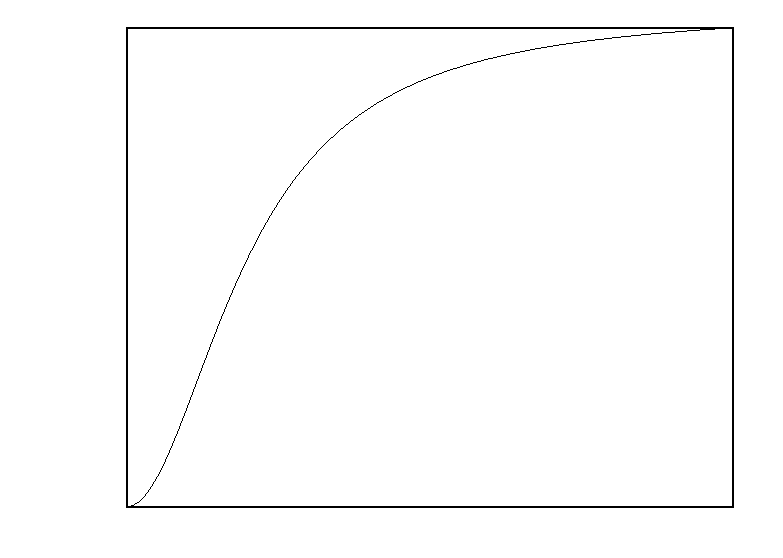
\includegraphics[width=5.5cm,height=4cm]{basic/growth.eps}}
	\caption{The course of knowledge development as observed in psychological and evolutionary data.}
	\label{f:st:growth}
\end{figure}

\begin{figure}
	\centering
	\subfigure[Word-forms]{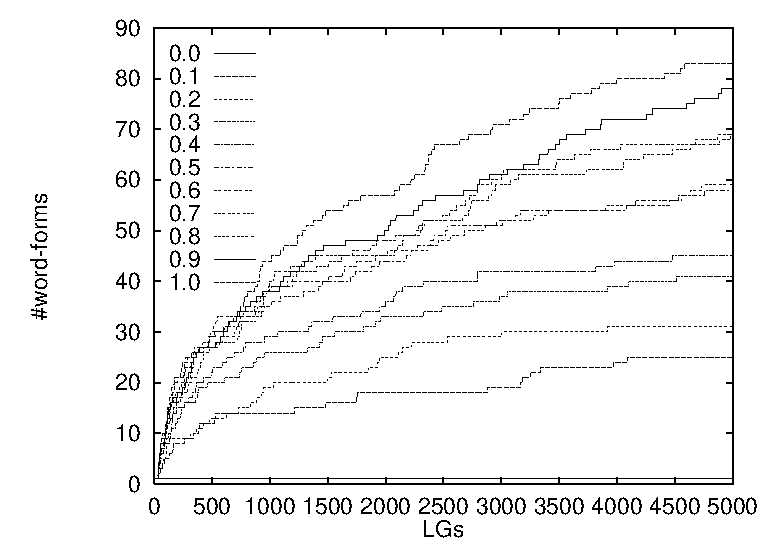
\includegraphics[width=.45\textwidth]{basic/words.eps}}
	\subfigure[Meanings]{\includegraphics[width=.45\textwidth]{basic/concepts.eps}}
	\caption{The average growth of the word-forms (a) and meanings (b) from the experiments. The growth is taken over elements that are used successfully in the language games.}
	\label{f:st:growthlex}
\end{figure}

\newpage The number of meanings that are used keep on growing, although slower than in the beginning. \figref{f:st:growthlex} (b) actually shows that the 8 word-forms that have been used successfully are associated with approximately 100 meanings. So, every word-form is associated with on the average 12.5 meanings. The semiotic landscape shown in above shows that this need not be a big problem.
\is{ontology!growth|)}
\is{lexicon!growth|)}
\is{lexicon|)}

\subsection{More language games}\label{s:st:10000}

The experiment introduced was done with 10 runs of 5,000 language games. Most experiments that are discussed have 10 runs of 5,000 language games, but what happens when the experiment is run for a longer time. \figref{f:st:10000} shows the results when the robots play 10,000 games each run (again for 10 runs). As is clear the system keeps on improving slightly. The communicative success for instance increases towards a value of 0.5. Also the specificity is increasing continuously. So, the communication system seems to keep on learning, but slowly.

It is unknown exactly when the slight growth stops, but the system does seem to stabilise towards the end. As will be shown in later chapters, some experiments will stabilise before 10,000 games are played.

\enlargethispage{4\baselineskip}
\begin{figure}[H]
\centering
\subfigure[CS]{\includegraphics[width=.45\textwidth]{basic/cs10.eps}}
\subfigure[DS]{\includegraphics[width=.45\textwidth]{basic/ds10.eps}}\\
\subfigure[S]{\includegraphics[width=.45\textwidth]{basic/spec10.eps}}
\subfigure[D]{\includegraphics[width=.45\textwidth]{basic/dist10.eps}}
\end{figure}
\begin{figure}[H]
\centering
\subfigure[C]{\includegraphics[width=.45\textwidth]{basic/cons10.eps}}
\subfigure[P]{\includegraphics[width=.45\textwidth]{basic/pars10.eps}}
\caption{The evolution of the basic experiment with runs of 10,000 language games.}
\label{f:st:10000}
\end{figure}


\section{Summary}\label{basic:summary}

This chapter introduced the first experimental results in detail. The experiment that has been presented here in detail will be used as the basic experiment from which parameters and methods are varied and with which the results of other experiments shall be compared. The experimental results of the forthcoming experiments will not be presented at the same level of detail. For most experiments only the global averages will be given. When appropriate, however, the results will be presented in more detail. 

The basic experiment used a data set that has been recorded in advanced  and that is used to process in different runs under different random seeds. The results have been presented with several measures, notably the communicative success, discriminative success, distinctiveness, specificity, parsimony and consistency. Although the communicative success is rather low, it is higher than the a priori communicative success. Furthermore, inspecting the other measures, it appeared that the robots did learn a reasonable communication system. Competition diagrams showed how the robots evolve to select preferred elements of their ontology and lexicon to name the referents. The semiotic landscape showed that one-to-many relations between referent and meaning need not be a problem as long as the polysemy is low.  However, the system still carries quite some polysemy and synonymy. 

The next chapters will show if and how a better communication system may emerge. First the impact from different methods and parameter settings \chapref{ch:cat}. Chapter \ref{ch:opt} reports some optimised systems.